% ═════════════════════════════════════════════════════════════
% A2 --- QR Factorization Experiments
\label{sec:qr_exp}
% ═════════════════════════════════════════════════════════════
\noindent This chapter evaluates the QR approach of Chapter~\ref{sec:qr} on the
same ML-CUP25 instance used for L-BFGS: $X\in\R^{m\times n}$ with $m=500$ and
$n=12$, the response vector $y$ drawn with the same fixed seed, and default
regularization $\lambda=0.5$ ($\kappa_2(A)\approx151$). We compare three
solvers for the same least-squares problem: the dense Householder QR of the
augmented matrix, which ignores its block structure; the structure-based
Householder QR of Section~\ref{sec:structured_householder}, which is the
solver proposed for this project; and the normal equations
$(XX^T+\lambda^2I_m)\,w=Xy$ solved with \texttt{numpy.linalg.solve}, used as
an external baseline.

\noindent Before any timing or stability study, we verify that the
implementation is correct on the default instance. A single Householder
reflector annihilates the subdiagonal part of its column and is orthogonal to
working precision (errors of order $10^{-16}$). Measured against an
independent SVD reference, both QR solvers reach a relative error of about
$4 \times 10^{-15}$, while the normal-equations solution is already at
$5 \times 10^{-13}$, a first sign of its squared condition number. Finally,
the implicit products with $Q$ and $Q^T$ are exact to working precision: for
both solvers $\norm{Q(Q^Tv) - v}/\norm{v}$ and the relative error of the
reconstruction $Q\,[R;0] = A$ are below $10^{-15}$, and for the
structure-based solver the norm of the trailing part of $Q^T\tilde b$ matches
the minimal residual to $6 \times 10^{-17}$, without ever forming $Q$.

\noindent Each reported time is the median of ten runs after a discarded
warm-up run, and data generation and accuracy diagnostics are always excluded
from the timed regions.

\noindent The chapter is organised in two parts. We first study the
\emph{computational cost} of the structure-based solver: a detailed operation
count, its asymptotic comparison with dense QR and the normal equations, and
the measured runtimes for increasing problem size $m$
(Section~\ref{sec:qr_scalability}). We then study its \emph{numerical
stability} as the conditioning of the problem is varied through $\lambda$,
comparing forward errors and optimality residuals against an independent SVD
reference (Section~\ref{sec:qr_stability}).


\section{Runtime Scalability}
\label{sec:qr_scalability}
\subsection{Detailed Operation Count}
\label{sec:qr_flop_count}

\noindent We now give a precise floating-point operation (FLOP) count for the
structure-based solver, beyond the asymptotic order, counting one flop per
floating-point addition or multiplication as for L-BFGS
(Section~\ref{sec:exp_cost}). At step $k$ the active
block is $(n+1)\times(m-k+1)$, and the work splits into three phases.

\paragraph{Reflector construction:} Computing the compact Householder vector
$u_k$ from the first column (length $n+1$) requires scaling, one Euclidean
norm, a sign choice, and a normalisation:
\[
  \text{build}(u_k) \;\approx\; 6(n+1) \ \text{FLOP},
\]
independent of the column index $k$. Over all $m$ columns this contributes
$6(n+1)\,m$, linear in $m$.

\paragraph{Block update:} Applying $H_k = I - 2u_ku_k^T$ to the active block
of width $w_k = m-k+1$ is the dominant cost. The product $u_k^T B_k$ costs
$2(n+1)w_k$, the outer product and the rank-one subtraction cost a further
$2(n+1)w_k$, for
\[
  \text{update at step } k \;\approx\; 4(n+1)(m-k+1) \ \text{FLOP}.
\]
Summing over $k=1,\dots,m$,
\[
  \sum_{k=1}^{m} 4(n+1)(m-k+1)
  \;=\; 4(n+1)\frac{m(m+1)}{2}
  \;\approx\; 2(n+1)\,m^2 \ \text{FLOP},
\]
which is the leading term of the factorisation.

\paragraph{Right-hand side and solve:} Applying the $m$ stored reflectors to
$\tilde b$ touches only an $(n+1)$-vector at each step, costing
$\approx 7(n+1)\,m$ in total; the final back-substitution on the $m\times m$
triangular factor costs $m^2$. Both are dominated by the factorisation for
$m \gg n$.

\paragraph{Total:} Collecting the three phases,
\begin{equation}
\label{eq:qr_flop_total}
  \text{FLOP}_{\text{struct}}(m,n)
  \;\approx\; \underbrace{2(n+1)m^2}_{\text{factorisation}}
           + \underbrace{m^2}_{\text{back-subst.}}
           + \underbrace{13(n+1)m}_{\text{reflectors + rhs}}
  \;=\; \bigl(2(n+1)+1\bigr)m^2 + O(nm).
\end{equation}
With $n=12$ the leading constant is $2(n+1)+1 = 27$, so the solver performs
about $27\,m^2$ FLOP. Table~\ref{tab:qr_flop_count} evaluates
Eq.~\eqref{eq:qr_flop_total} at the sampled sizes.

\begin{table}[H]
\centering
\caption{Theoretical FLOP counts ($n = 12$): structure-based QR from
  Eq.~\eqref{eq:qr_flop_total}; dense Householder QR of the $(m+n)\times m$
  augmented matrix, ${\approx}\,2(m+n)m^2-\tfrac23 m^3$; normal equations
  solved by LU as in \texttt{numpy.linalg.solve}, ${\approx}\,2nm^2+\tfrac23 m^3$.
  The last column is the ratio normal equations / structure-based.}
\label{tab:qr_flop_count}
\small
\setlength{\tabcolsep}{8pt}
\begin{tabular}{rrrrr}
    \toprule
    $m$ & \textbf{Structure-based} & \textbf{Dense QR} & \textbf{Normal eq.}
        & \textbf{Ratio} \\
    \midrule
     100 & $2.9 \times 10^{5}$ & $1.6 \times 10^{6}$  & $9.3 \times 10^{5}$  & $3.2\times$ \\
     500 & $6.8 \times 10^{6}$ & $1.7 \times 10^{8}$  & $9.0 \times 10^{7}$  & $13.1\times$ \\
    1000 & $2.7 \times 10^{7}$ & $1.4 \times 10^{9}$  & $6.9 \times 10^{8}$  & $25.5\times$ \\
    2000 & $1.1 \times 10^{8}$ & $1.1 \times 10^{10}$ & $5.4 \times 10^{9}$  & $50.2\times$ \\
    4000 & $4.3 \times 10^{8}$ & $8.6 \times 10^{10}$ & $4.3 \times 10^{10}$ & $99.6\times$ \\
    \bottomrule
\end{tabular}
\end{table}

\noindent The count makes the structural advantage quantitative rather than
asymptotic. Both the structure-based solver and the normal equations share
the $O(nm^2)$ term from touching the dense block, but the normal equations
add a cubic $\tfrac23 m^3$ term from the dense LU factorisation, and dense QR
an even larger one, both absent here because the $\lambda I_m$ block is
already triangular. The resulting advantage grows with $m$: from about
$3\times$ at $m=100$ to about $100\times$ at $m=4000$ over the normal
equations, matching the $O(nm^2)$ versus $O(m^3)$ gap of
Eq.~\eqref{eq:qr_scaling_summary}.

\subsection{Asymptotic Cost and Timings}
\noindent The column-oriented structure-based method applies one reflector to an
$(n+1)\times(m-k+1)$ block at each step. Its factorization cost is therefore $\sum_{k=1}^{m}O\bigl((n+1)(m-k+1)\bigr)=O(nm^2+m^2)$.

\noindent Applying the reflectors to the right-hand side costs $O(nm)$ and back
substitution costs $O(m^2)$. The complete structure-based solver thus costs

\begin{equation}
    O(nm^2 + m^2).
\end{equation}

\noindent Combining these bounds with Section~\ref{sec:qr_cost_project} gives

\begin{equation}
\label{eq:qr_scaling_summary}
\begin{aligned}
    T_{\mathrm{dense\ QR}}(m,n) &= O(m^3+nm^2),\\
    T_{\mathrm{structure\text{-}based\ QR}}(m,n) &= O(m^2+nm^2),\\
    T_{\mathrm{normal\ equations}}(m,n) &= O(m^3+nm^2).
\end{aligned}
\end{equation}

\noindent Hence, with the project value $n=12$ fixed, the structure-based algorithm is quadratic in $m$, whereas generic dense QR and a dense normal-equations solve retain a cubic term.

\begin{figure}[H]
    \centering
    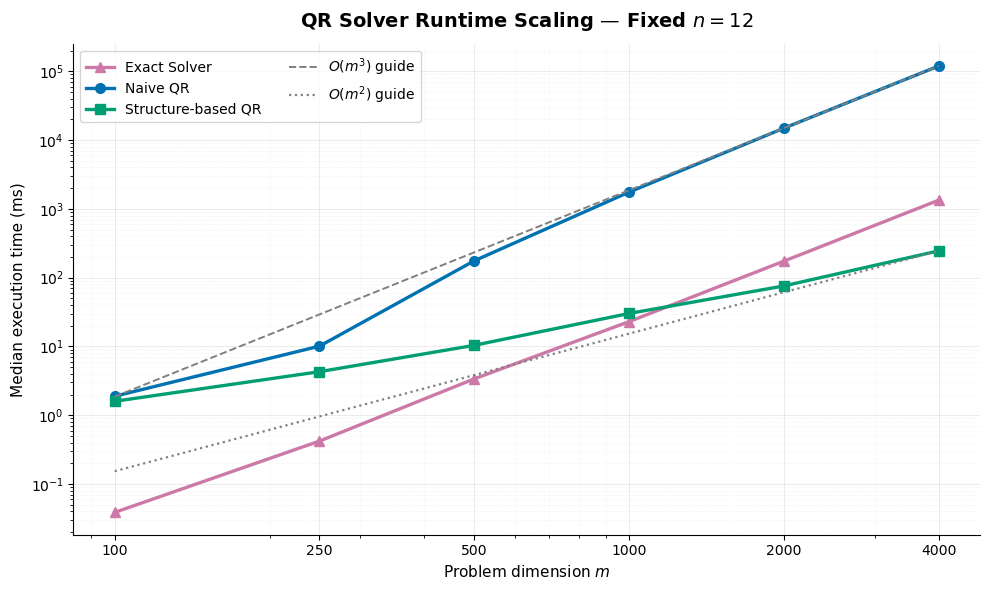
\includegraphics[width=0.50\textwidth]{Chapters/images/qr_runtime_scaling.png}
    \caption{Median solver times for increasing $m$, with $n=12$ fixed.}
    \label{fig:qr_runtime_scaling}
\end{figure}

\noindent The structure-based implementation stores the triangular factor, a copy of the dense block, and $m$ reflectors of length $n+1$, for $O(m^2+nm)$ memory. 
% The current row-insertion wrapper also stores all $nm$ two-dimensional reflector records; disabling that optional storage would leave only $O(m)$ workspace in addition to $R$.

\noindent The notebook first constructs a single matrix with $4000$ rows. The original $500$ rows are retained as the leading block; each additional row is sampled as a complete row of $X$ and perturbed by Gaussian noise scaled by the empirical standard deviation of each column. Taking prefixes of this matrix produces nested problems with fixed $n=12$, $m\in\{100,250,500,1000,2000,4000\}$, and $\lambda=0.5$. Data generation is performed once, outside every timed region. Each entry in Table~\ref{tab:qr_runtime_scaling} is the median of ten runs after a discarded warm-up run.

\begin{table}[H]
\centering
\caption{Internal solver times in milliseconds for the augmented-data runtime
sweep. The normal-equations timer is partial.}
\label{tab:qr_runtime_scaling}
\small
\setlength{\tabcolsep}{8pt}
\begin{tabular}{rrrr}
    \toprule
    $m$ & \textbf{Normal eq.} & \textbf{Dense QR}
        & \textbf{Structure-based QR}\\
    \midrule
     100 &    0.039 &      1.891 &   1.596\\
     250 &    0.421 &     10.094 &   4.296\\
     500 &    3.379 &    175.910 &  10.392\\
    1000 &   22.975 &   1754.163 &  30.200\\
    2000 &  174.064 &  14927.239 &  75.879\\
    4000 & 1340.009 & 119515.903 & 245.618\\
    \bottomrule
\end{tabular}
\end{table}

\noindent The QR timings include the preparation of the required data structures, factorization, transformation of the right-hand side, and back substitution. Dataset generation and accuracy diagnostics are excluded from the timed regions. The normal-equations timer, instead, covers only \texttt{numpy.linalg.solve}
and excludes the formation of $XX^T+\lambda^2I_m$ and $Xy$, which favours
this baseline.

\noindent Figure~\ref{fig:qr_runtime_scaling} highlights the growing runtime
gap between dense QR and the structure-based method, which is the faster of
the two QR solvers at every sampled size, reaching a speedup of about
$487\times$ over dense QR at $m=4000$. The cubic versus quadratic separation
is clear on the final doubling from $m=2000$ to $m=4000$: dense QR and the
normal equations grow by factors of about $8.0$ and $7.7$, close to the
$2^3=8$ expected of an $O(m^3)$ method, against the $3.2$ of structure-based
QR, below the $2^3$ of a cubic method and approaching the $2^2=4$ of an
$O(m^2)$ one, consistent with Eq.~\eqref{eq:qr_scaling_summary}.

\noindent The detailed operation count of Section~\ref{sec:qr_flop_count}
predicts a leading term of $\bigl(2(n+1)+1\bigr)m^2 \approx 27\,m^2$
floating-point operations for $n=12$, so the work quadruples on each doubling
of $m$. The measured times grow more slowly, by factors between $2.5$ and
$3.2$ from $m=500$ to $m=4000$: the time per predicted flop decreases from
about $1.5$ to $0.6$\,ns. The solver executes a Python loop over the $m$
columns, each step paying a fixed interpretation overhead and acting on a
block of only $n+1=13$ rows; as $m$ grows, the blocks become wider, the
overhead is amortised and the arithmetic dominates. The quadratic growth
predicted by the model is therefore approached from below, and becomes
apparent at the largest sizes.

\noindent The normal equations are faster than the structure-based solver up
to $m = 1000$, and slower from $m = 2000$ onwards, by $2.3\times$ at
$m = 2000$ and $5.5\times$ at $m = 4000$, a gap that grows with $m$ as the
flop count predicts. At small $m$ their advantage has two sources: their timer
is partial, as noted above, and \texttt{numpy.linalg.solve} runs a compiled,
blocked LAPACK factorization that executes far more operations per second than
our Python loop. As $m$ grows, however, their cubic term outweighs this
efficiency: flop counts do not predict the absolute ratio between
implementations of different nature, but they do predict how it evolves.

\section{Algorithmic Stability and the Condition Number}
\label{sec:qr_stability}

\noindent Conditioning is a property of the mathematical problem, whereas
stability is a property of the algorithm used to solve it. For
$A=[X^T;\lambda I_m]$,

\begin{equation}
    A^T A=XX^T+\lambda^2I_m.
\end{equation}

\noindent Given $\lambda>0$, the condition number of $A$ is

\begin{equation}
\label{eq:qr_condition_lambda}
\begin{aligned}
    \kappa_2(A)
    = \|A\|_2 \|A^\dagger\|_2
    = \frac{\sigma_{\max}(A)}{\sigma_{\min}(A)}
    = \sqrt{
        \frac{\lambda_{\max}(XX^T+\lambda^2I_m)}
             {\lambda_{\min}(XX^T+\lambda^2I_m)}
       }
    = \frac{\sqrt{\sigma_{\max}(X)^2+\lambda^2}}{\lambda}.
\end{aligned}
\end{equation}

\noindent The singular values of $A$ are the square roots of the
eigenvalues of $A^TA=XX^T+\lambda^2I_m$.
Since $m>n$, $XX^T$ has a zero eigenvalue, hence
$\lambda_{\min}(A^TA)=\lambda^2$, the eigenvalue shift introduced
by regularization.

\noindent If $X\neq0$, Eq.~\eqref{eq:qr_condition_lambda} behaves as
$\sigma_{\max}(X)/\lambda$ when $\lambda\to0^+$ and tends to $1$ as
$\lambda\to\infty$. Forming the normal equations squares this number, as
shown in Eq.~\eqref{eq:qr_condition_squaring}; this is precisely the
conditioning penalty avoided by Householder QR, getting $\kappa_2(A)$ instead of $\kappa_2(A)^2$.

\noindent In the standard floating-point model with machine precision
$\varepsilon_{\mathrm{mach}}$, Householder QR is backward stable: up to
dimension-dependent constants, the computed factors are the exact QR factors
of $A+\Delta A$ with

\begin{equation}
    \frac{\norm{\Delta A}_2}{\norm{A}_2}=O(\varepsilon_{\mathrm{mach}}),
\end{equation}

\noindent and the computed orthogonal factor is orthogonal to working precision. The resulting forward error still depends on the conditioning and geometry of the least-squares problem. Accordingly, the notebook uses $\varepsilon_{\mathrm{mach}} \kappa_2(A)$ for Householder QR and $\min\{1,\varepsilon_{\mathrm{mach}} \kappa_2(A)^2\}$ for the normal equations as heuristic indicators of the expected forward-error scale. These quantities should not be interpreted as rigorous universal upper bounds. In particular, the forward sensitivity of a least-squares solution depends not only on $\kappa_2(A)$, but also on the geometry of the problem, including the size and orientation of the residual. The curves are therefore intended only to illustrate the expected conditioning trend of the two methods. The notebook additionally plots $\varepsilon_{\mathrm{mach}}$ as a reference scale for $\eta_{\mathrm{opt}}$.

\noindent The notebook diagnoses this behavior using an independent thin-SVD
reference. If $X=U\Sigma V^T$, then the Tikhonov solution is

\begin{equation}
\label{eq:qr_svd_reference}
    w_{\mathrm{SVD}}
    =U\operatorname{diag}\!\left(
        \frac{\sigma_i}{\sigma_i^2+\lambda^2}
      \right)V^T y.
\end{equation}

\noindent For a computed solution $w$, the two reported diagnostics are the
relative forward error

\begin{equation}
\label{eq:qr_forward_error}
    e_{\mathrm{fwd}}
    =\frac{\norm{w-w_{\mathrm{SVD}}}_2}{\norm{w_{\mathrm{SVD}}}_2}
\end{equation}

\noindent and, for the augmented residual $r=Aw-b\neq0$, the scaled first-order
optimality residual

\begin{equation}
\label{eq:qr_scaled_optimality}
    \eta_{\mathrm{opt}}
    =\frac{\norm{A^T r}_2}{\norm{A}_2\norm{r}_2}.
\end{equation}

\noindent At an exact least-squares solution $A^T r=0$, so a small
$\eta_{\mathrm{opt}}$ verifies the optimality condition. It does not by itself
guarantee a small forward error when $A$ is severely ill-conditioned; both
diagnostics must therefore be considered together.

\begin{figure}[H]
    \centering
    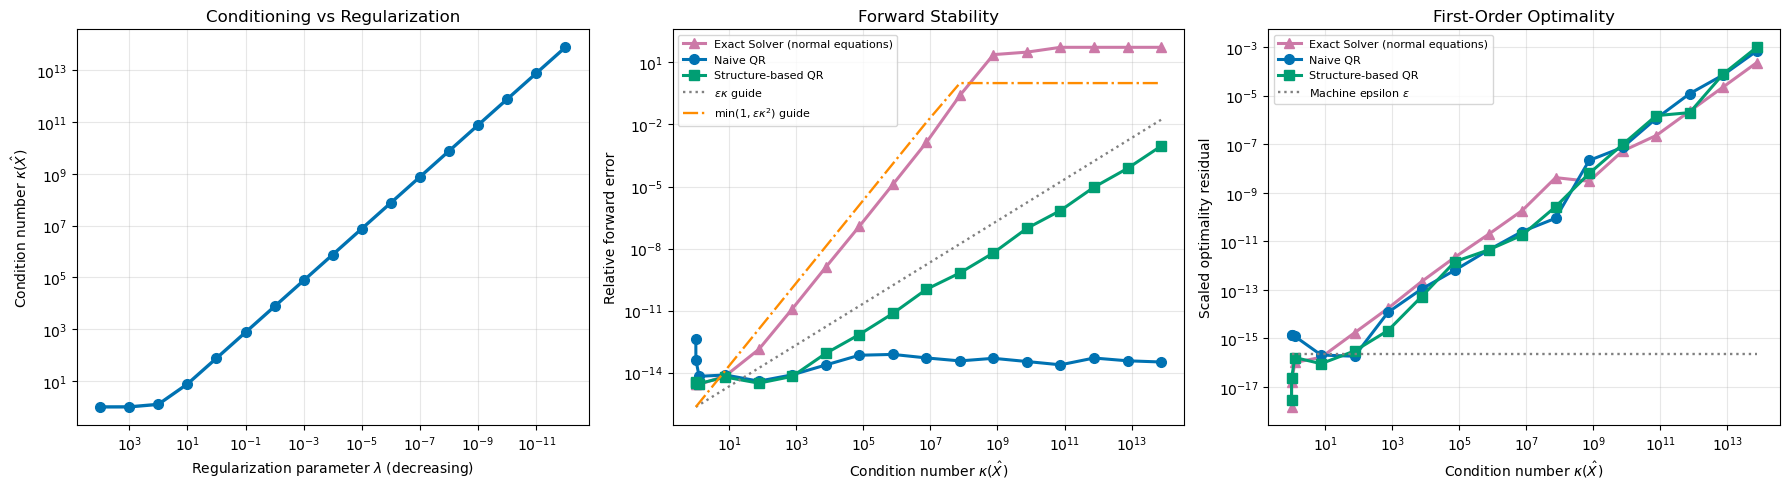
\includegraphics[width=\textwidth]{Chapters/images/qr_conditioning_stability.png}
    \caption{Conditioning and numerical stability: condition number versus
    $\lambda$ (left), relative forward error (middle), and scaled optimality
    residual (right).}
    \label{fig:qr_conditioning_stability}
\end{figure}

\noindent The experiment in Figure~\ref{fig:qr_conditioning_stability} sweeps $\lambda\in\{10^j:j=-12,\ldots,4\}$.
The left panel shows the growth of the condition number as $\lambda$ decreases, from $\kappa_2(A)\approx1$ at
$\lambda=10^4$ to $\kappa_2(A)\approx7.6\times10^{13}$ at $\lambda=10^{-12}$.
The middle panel shows that the normal equations lose accuracy much earlier than both Householder methods. 
At $\lambda=10^{-6}$
($\kappa_2(A)\approx7.6\times10^{7}$) the normal equations already have a
relative forward error of $2.5\times10^{-1}$, so that not even the leading digit is reliable, whereas
structure-based QR attains $6.7\times10^{-10}$. At $\lambda=10^{-12}$ the
normal-equations error saturates around $54$, while structure-based QR still
retains about three correct digits ($9.0\times10^{-4}$).

\noindent To make this conditioning penalty quantitative, we fit the forward
error against $\kappa_2(A)$ in log--log scale over the intermediate range
$\kappa_2(A)\in[10^4,10^8]$, large enough for the error to grow but below the
saturation of the normal equations. The fitted slopes are $2.10$ for the normal
equations and $1.01$ for structure-based QR, recovering the theoretical
exponents: forming $A^TA$ makes the error grow as $\kappa_2(A)^2$
(Eq.~\eqref{eq:qr_condition_squaring}), whereas QR works directly with the
triangular factor and degrades only as $\kappa_2(A)$.

\noindent Dense QR behaves differently: its forward error remains at the
$10^{-14}$ level throughout the ill-conditioned regime (fitted slope
$\approx 0$), and never exceeds $5\times10^{-13}$ over the whole sweep.
Retaining all $m+n$ rows makes
it the most accurate method in the ill-conditioned regime, but its $O(m^3)$
cost (Section~\ref{sec:qr_scalability}) makes it impractical for large $m$.
This near-machine-precision behaviour is an empirical property of this problem
and should not be read as a conditioning-independent guarantee. The
structure-based solver therefore trades a modest amount of accuracy, growing
as $\varepsilon_{\mathrm{mach}}\kappa_2(A)$, for a cost that is quadratic rather
than cubic in $m$, while remaining dramatically more accurate than the normal
equations.

\noindent The right panel shows why the two diagnostics must be read together.
At $\lambda=10^{-12}$ the normal equations attain the \emph{smallest} scaled
optimality residual of the three solvers ($2.3\times10^{-4}$), yet their
forward error at the same point is the \emph{largest} by many orders of
magnitude. A small $\eta_{\mathrm{opt}}$ certifies that $A^Tr\approx0$ for the
computed solution, but on a severely ill-conditioned problem this does not
imply closeness to the true minimiser: the normal equations accurately solve a
perturbed problem while landing far from $w_{\mathrm{SVD}}$. The forward error
is therefore the decisive diagnostic, and by that measure both Householder
methods dominate the normal equations across the ill-conditioned range.

% ═════════════════════════════════════════════════════════════
\section{Summary}
\label{sec:qr_summary}
% ═════════════════════════════════════════════════════════════

\noindent Our experiments confirm that exploiting the block structure of the
augmented matrix makes Householder QR both cheaper and, compared with the
normal equations, far more robust, as predicted in Chapter~\ref{sec:qr}.

\noindent On the side of \emph{computational cost}, the detailed operation count
shows that the structure-based solver performs about $27\,m^2$ flops for
$n=12$, with no cubic term, because the $\lambda I_m$ block is already
triangular and every reflector has fixed length $n+1$. Dense QR and the
normal equations instead retain a cubic term, so the theoretical advantage
grows linearly with $m$, from about $3\times$ to about $100\times$ over the
normal equations in the sampled range. The measured runtimes follow these predictions: on the final doubling from
$m=2000$ to $m=4000$, dense QR and the normal equations grow by about $8.0$
and $7.7$, and the structure-based solver by about $3.2$. At $m=4000$ the
structure-based solver is about $487\times$ faster than dense QR.
Its growth approaches the quadratic rate from below, because the fixed cost
of its Python loop over the columns is amortised as $m$ grows. The normal
equations, which run in compiled LAPACK code and are timed only partially,
are faster up to $m=1000$; from $m=2000$ onwards the cubic term dominates, and
the structure-based solver becomes faster, by $5.5\times$ at $m=4000$.

\noindent On the side of \emph{numerical stability}, the sweep over $\lambda$
shows the effect of the condition-number squaring of the normal equations.
At $\lambda=10^{-6}$ ($\kappa_2(A)\approx7.6\times10^{7}$) the normal
equations no longer have a reliable leading digit, whereas the
structure-based solver attains a relative forward error of
$6.7\times10^{-10}$; at $\lambda=10^{-12}$ it still retains about three
correct digits, while the normal-equations error has saturated. A log--log
fit recovers the theoretical exponents, with slopes $2.10$ for the normal
equations and $1.01$ for structure-based QR. Dense QR is the most accurate
method, remaining at the $10^{-14}$ level, but at an $O(m^3)$ cost. The
structure-based solver therefore offers the best trade-off: quadratic cost in
$m$ and an error that grows only as $\varepsilon_{\mathrm{mach}}\kappa_2(A)$.
Finally, a small scaled optimality residual alone does not certify an
accurate solution on ill-conditioned problems, so both diagnostics must be
read together.